\documentclass[]{article}
\usepackage{amssymb}
\usepackage[backend=bibtex,style=authoryear,natbib=true]{biblatex} % Use the bibtex backend with the authoryear citation style (which resembles APA)

\addbibresource{example.bib} % The filename of the bibliography

\usepackage[autostyle=true]{csquotes} % Required to generate language-dependent quotes in the bibliography

\usepackage{tikz}
\usepackage{tikz-network}
\usepackage{breqn}
\usepackage{bm}
\usepackage{graphicx}
\usepackage{subcaption}
\usepackage{multirow}
\usetikzlibrary{fit}
\usetikzlibrary {arrows.meta,graphs,shapes.misc}
\usetikzlibrary {positioning}

\newcommand{\bn}{\textbf{n}}
\newcommand{\tabhead}[1]{\textbf{#1}}

\begin{document}
	
\section{Guided normal inference using GCNN}

\subsection{Shape from shading}
Intrinsic image model was introduced by \cite{intrinsic-image}. It represents that an image $ I $ can be decomposed as the element-wise product between the reflectance $ R $ of the object and the shading $ S $ produced by the interaction between light and objects.
\[ I =R  \odot S\]
The equation can be further decomposed based on different surface models. If assume the object surfaces are Lambertian surfaces, i.e. the diffuse surfaces, the equation can be decomposed further as follows
\[ I = \rho  \odot (L_0 \textbf{L} \cdot  \textbf{N}) \]
where $ \rho $ is the reflectance of diffuse surface, also know as albedo, $ L_0 $ is the radiance of  incoming light, i.e. irradiance, $ \textbf{L} $ is the opposite direction of incoming light as unit vector map and $ \textbf{N} $ is the surface normal also as unit vector map, as shown in Figure \ref{fig:lambertian-surface}

\begin{figure}[th]
	\centering
	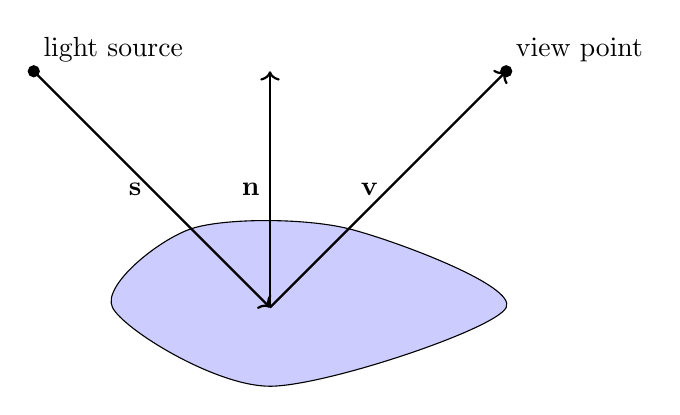
\begin{tikzpicture} 
		% reference lines
		\draw [fill=blue!20] plot [smooth cycle] coordinates {(0,0) (1,1) (3,1) (5,0) (2,-1)}; %% surface element
		\draw[thick, ->] (2,0) -- (2,3) node[midway, left] {$ \textbf{n} $}; %% normal
		\draw[thick, ->] (-1,3) -- (2,0) node[midway, left] {$ \textbf{s} $}; %% source direction
		\draw[thick, ->] (2,0) -- (5,3) node[midway, left] {$ \textbf{v} $}; %% view direction
		\filldraw[black] (-1,3) circle (2pt) node[anchor=south west]{light source}; %% light source
		\filldraw[black] (5,3) circle (2pt) node[anchor=south west]{view point}; %% view point		
	\end{tikzpicture}	
	\caption{Lambertian Surface}
	\label{fig:lambertian-surface}
\end{figure}

The equation can be further rearranged as follows
\[ I = \textbf{g} \cdot \textbf{L} =(L_0\rho \odot \textbf{N}) \cdot  ( \textbf{L}) \]
The shape from shading method employed the equation mentioned above to predict the both surface albedo and the normal. More specifically, a set of $ k $ image for the same scene have been captured based on different light projections. Then, for each pixel $ (x,y) $ in the image, an equation system can be set up 

\[ 
\begin{pmatrix}
	L_1^T \\
	L_2^T \\
	\cdots \\
	L_k^T
\end{pmatrix} g(x,y) = 
\begin{pmatrix}
	I_1(x,y) \\
	I_2(x,y) \\
	\cdots \\
	I_3(x,y)
\end{pmatrix}
\]
for the simplicity, $ L_i^T $ for $ 1\le i \le k $ denotes the light direction at position $ (x,y) $ in the image $ k $ 
The equation can be solved based on least square methods. 
Since normal $ N(x,y) $ is unit vector, thus we have 

\[ \|g(x,y)\|_2 = \|L_0\rho(x,y)N(x,y)\|_2 = L_0\rho(x,y) \]

Then the normal can be obtained as follow

\[  N(x,y) = \frac{g(x,y)}{L_0\rho(x,y)}\]

In another word, the surface normal including the albedo can be obtained directly based on images and light directions. 


\subsection{Light and image guided normal inference using GCNN}


The decomposition gives a constraint of the normal map with given other information, which can be considered further in the deep learning model. The image $ I $ is given in the RGB-D image, the light map $ \textbf{L} $ can be calculated based on the light source and the vertex map. 

Inspired by the Shape from shading approach mentioned above, a new approach is proposed in this thesis for normal prediction. The structure is shown in Figure \ref{fig:albedo-gated-archi}. The model takes image $ \textbf{I} $, Light direction $ \textbf{L} $ and 3D vertex $ \textbf{V} $ as input. Each input has its own branch based on UNet architecture with four times fusion in the upsampling part. 





\subsection{Light Map}
The incoming light direction of each point can be represented as a matrix with same size as normal map or vertex map, where each pixel corresponding with each other.

%% calc the light direction matrix
\paragraph{Calculation}
The incoming light direction can be calculated based on the position of light source and points. As shown in Figure \ref{fig:lambertian-surface-principle}, the incoming light direction of the surface point is a vector point from light source to the surface point, therefor it can be calculated as follows

\begin{equation}\label{light-direction}
	\begin{array}{ll}
		L&= \frac{V-S}{\|V-S\|_2}\\ 
	\end{array}
\end{equation}
where $ S $ is the light source position and $ V $ is the vertices, both $ S $ and  $ V $ are with respect to the camera space. The light direction map $ L $ is normalized since only the direction of the light is considered. 

\paragraph{Inpainting}
Due to the exist noise in the vertex map, the getting light map is also semi-dense.

stores for every pixel the direction of incoming light.
find a mapping H, such that $ l_{in} = H(v, l_{s}) $ for pixel $ v $, $ l_s $ is the position of light source, $ l_{in} $ is direction of incoming light of pixel $ v $. Iterate all the pixels, we get the light direction map $ L $.



\end{document}
